\documentclass[tikz,border=5pt]{standalone}
\usepackage{tikz}
\usetikzlibrary{arrows.meta, positioning, fit}

\begin{document}

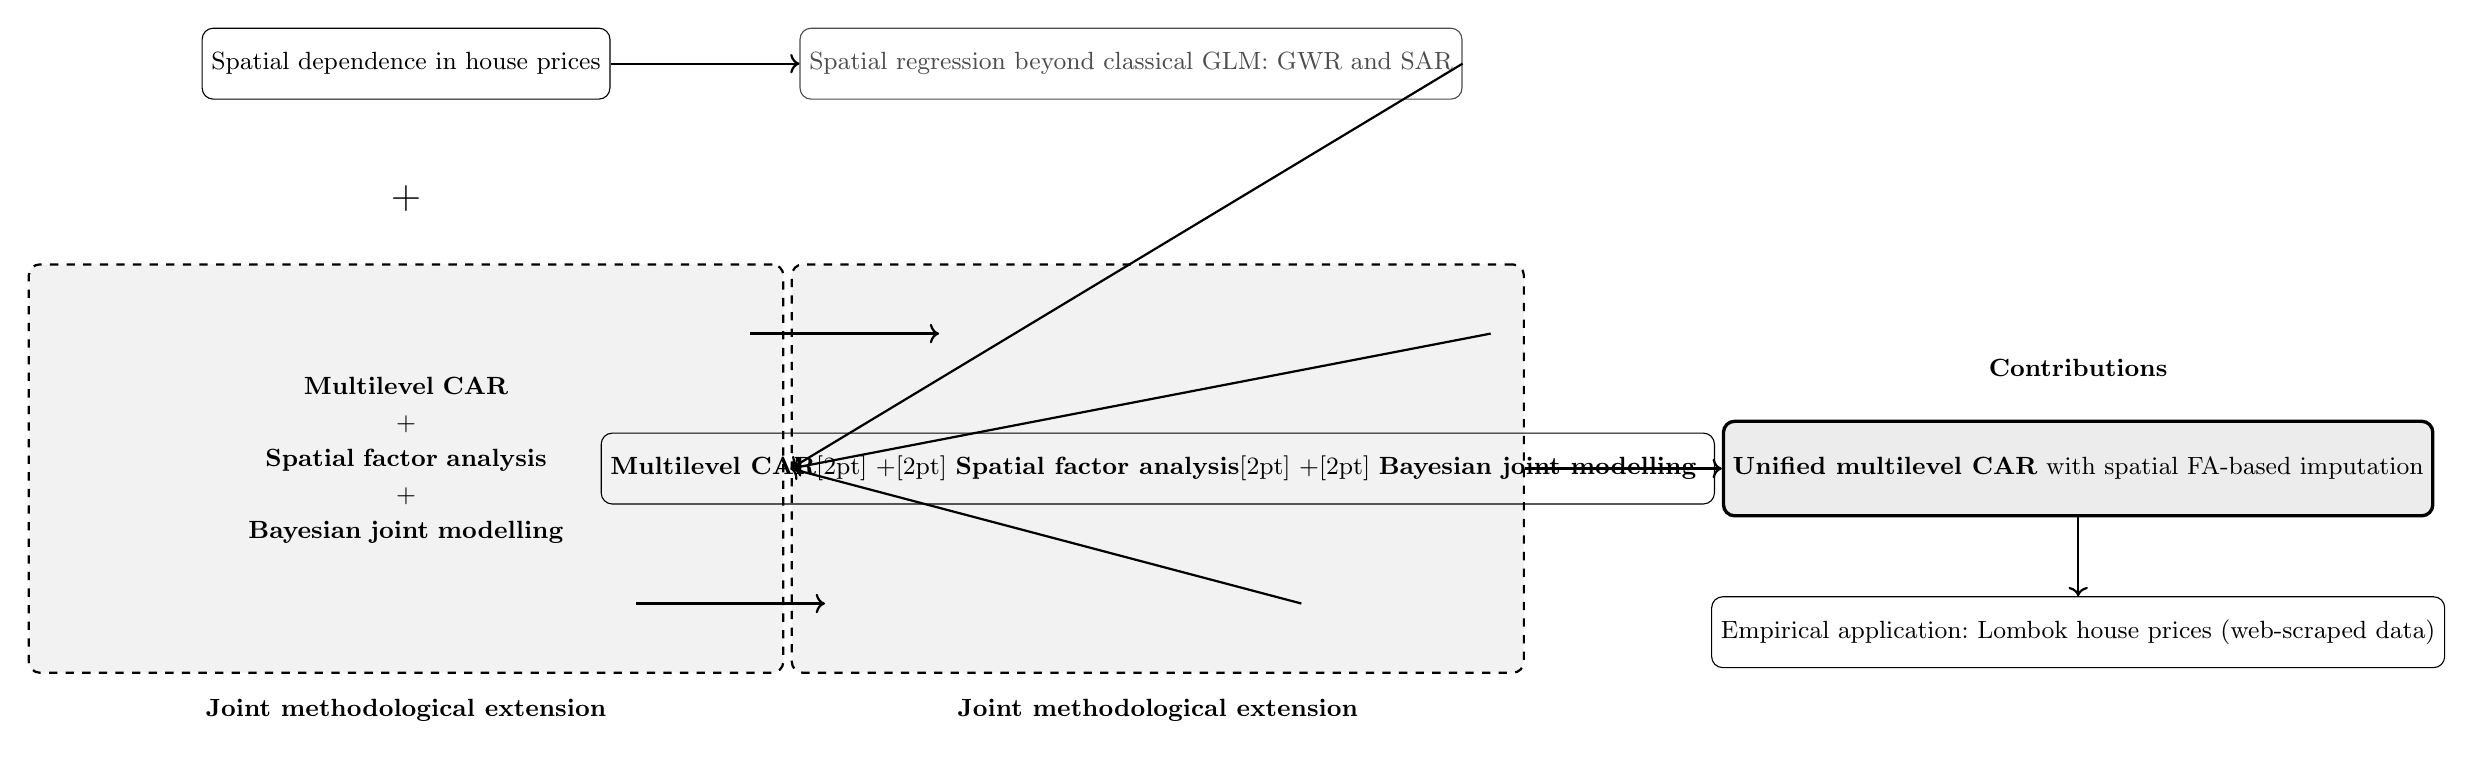
\begin{tikzpicture}[
every node/.style={
draw,
rounded corners,
align=center,
minimum width=5.0cm,
minimum height=9mm,
font=\small
},
arrow/.style={->, thick},
node distance=8mm
]

% ------------------------
% Housing data characteristics (left)
% ------------------------
\node (d1) {Spatial dependence\ in house prices};

\node[draw=none, below=of d1] (plus1) {\Large $+$};

\node (d2) [below=of plus1]
{Hierarchical data structure\ (multiple observations per area)};

\node[draw=none, below=of d2] (plus2) {\Large $+$};

\node (d3) [below=of plus2]
{Missing covariates\ in real-world listings};

\node[
    draw,
    dashed,
    thick,
    fill=gray!10,
    rounded corners,
    fit=(d2)(d3),
    inner sep=12pt,
    align=center,
    label=below:{\textbf{Joint methodological extension}}
] (methodbox) {
\textbf{Multilevel CAR}\\[2pt]
+\\[2pt]
\textbf{Spatial factor analysis}\\[2pt]
+\\[2pt]
\textbf{Bayesian joint modelling}
};

% ------------------------
% Methodological directions (middle)
% ------------------------
\node (m1) [right=24mm of d1, opacity=0.7]
{Spatial regression beyond classical GLM:\ GWR and SAR};

\node (m2) [right=24mm of d2]
{CAR and multilevel CAR\ modelling framework};

\node (m3) [right=24mm of d3]
{Spatially coherent\ missing data handling};

% Joint extension box
\node[
draw,
dashed,
thick,
fill=gray!10,
rounded corners,
fit=(m2)(m3),
inner sep=12pt,
label=below:{\textbf{Joint methodological extension}}
] (methodbox) {};

% Content inside method box
\node at (methodbox.center) {
\textbf{Multilevel CAR}[2pt]
+[2pt]
\textbf{Spatial factor analysis}[2pt]
+[2pt]
\textbf{Bayesian joint modelling}
};

% ------------------------
% Final contribution (right)
% ------------------------
\node (final) [
right=25mm of methodbox,
minimum width=6.5cm,
minimum height=12mm,
very thick,
fill=gray!15,
label={[label distance=2mm]above:{\textbf{Contributions}}}
]
{\textbf{Unified multilevel CAR}\
with spatial FA-based imputation};

% ------------------------
% Arrows (clean horizontal flow)
% ------------------------
\draw[arrow] (d1.east) -- (m1.west);
\draw[arrow] (d2.east) -- (m2.west);
\draw[arrow] (d3.east) -- (m3.west);

% Converging into method box
\draw[arrow] (m1.east) -- (methodbox.west);
\draw[arrow] (m2.east) -- (methodbox.west);
\draw[arrow] (m3.east) -- (methodbox.west);

% Final arrow
\draw[arrow] (methodbox.east) -- (final.west);

% ------------------------
% Empirical application (bottom)
% ------------------------
\node (lombok) [
below=10mm of final,
minimum width=6.0cm
]
{Empirical application:\ Lombok house prices\ (web-scraped data)};

\draw[arrow] (final) -- (lombok);

\end{tikzpicture}

\end{document}
